\section{Auswertung}
\subsection{Erhaltene Daten}.
MC Daten \\
echte Daten \\
Energien der echten Daten \\
Luminositäten \\
Strahlungskorrekturen 
\subsection{Bestimmung der Schnitte}
Reinheiten
\subsection{Berechnung der Effizienzmatrix}
Werden die oben bestimmten Schnitte auf die Monte-Carlo-Daten angewendet, kann man die Effizienz $\bm{E}$ der Schnitte berechnen. 
Die Effizienzmatrix gibt an, welcher Anteil der verschiedenen Ereignisse nach einem Schnitt noch vorhanden sind. Sie ist definiert als 
\begin{equation}
    \bm{E}_{ij} = \frac{n_{ij}^\text{cut}}{n_i} \ \, .
\end{equation} 
$i, j \in $ e$^+$e$^-$, \textmu$^+$\textmu$^-$, \texttau$^+$\texttau$^-$, q$^+$q$^-$ \\  %TODO format
Dabei bezeichnet $n_{ij}^\text{cut}$ die Anzahl der Ereignisse von Typ $i$ nach Schnitt von Typ $j$ und $n_i$ die gesamte Anzahl von Ereignissen 
der Monte-Carlo-Simulation von Typ $i$. 
Die Beziehung zwischen den Anzahlen von gemessenen Ereignissen nach Schnitt $\vec{M}$\footnote{"measurement"} und den echten Anzahlen 
$\vec{T}$\footnote{"truth"} lautet durch die Definition der Effizienzmatrix $\bm{E}$:
\begin{equation}
    \label{eq:effmat:mtrel}
    \vec{M} = \bm{E} \vec{T}
\end{equation}
Die Effizienzmatrix unsere Schnitte ist in \autoref{tab:effmat:val} dargestellt.
\begin{table}[H]
\caption{Effizienzmatrix.}
\begin{center}
\begin{tabular}{|c|c|c|c|c|}
  \hline
  Schnitt$\backslash$MC-Daten & \ee & \mm & \tt & \qq \\ \hline
  \ee & 0.388233 & 0.000011 & 0.001995 & 0.000010 \\ \hline
  \mm & 0.000160 & 0.890762 & 0.003585 & 0.000000 \\ \hline
  \tt & 0.001791 & 0.004259 & 0.747406 & 0.002354 \\ \hline
  \qq & 0.000000 & 0.000000 & 0.001868 & 0.966965 \\ \hline
\end{tabular}
\end{center}
\label{tab:effmat:val}
\end{table}

Nun gilt es den Fehler der einzelnen Einträge der Effizienzmatrix zu bestimmen. Hierzu wird die Definition der Effizienz $\epsilon$ leicht geändert:
\begin{equation}
    \epsilon = \frac{p}{p+f}	
\end{equation}
Die Anzahl der Ereignisse, die nach Schnitt noch da sind, wird mit $p$\footnote{"pass"} bezeichnet. Aus der totalen Anzahl $n$ der Ereignisse lässt 
sich die Anzahl derjenigen Ereignisse $f$\footnote{"fail"} berechnen, die beim Schnitt wegfallen. Da $p$ und $f$ als poissonverteilt angenommen 
werden können (bei hinreichenden Größen von $p$ und $f$), gilt für den Fehler der Effizienz mit Gauß'scher Fehlerfortpflanzung:
\begin{equation}
    s_\epsilon = \sqrt{\frac{f \cdot p}{ \left( f + p \right)^3}} \ \, .
\end{equation}
Mit der Definition von $\epsilon$ und $n$ kann man den Fehler zu der in der Literatur üblichen Form umformen:
\begin{equation}
    s_\epsilon = \sqrt{\frac{\epsilon (1-\epsilon)}{n}}
\end{equation}
Somit können nun die Fehler von den Einträge der Effizienzmatrix bestimmt werden (\autoref{tab:effmat:err}).
\begin{table}[H]
\caption{Fehler der Effizienzmatrix.}
\begin{center}
\begin{tabular}{|c|c|c|c|c|}
  \hline
  Schnitt$\backslash$MC-Daten & \ee & \mm & \tt & \qq \\ \hline
  \ee & 0.001591 & 0.000011 & 0.000159 & 0.000010 \\ \hline
  \mm & 0.000041 & 0.001015 & 0.000212 & 0.000000 \\ \hline
  \tt & 0.000138 & 0.000212 & 0.001544 & 0.000154 \\ \hline
  \qq & 0.000000 & 0.000000 & 0.000153 & 0.000569 \\ \hline
\end{tabular}
\end{center}
\label{tab:effmat:err}
\end{table}

\subsubsection{Berechnung der inversen Effizienzmatrix}
Wenn die Schnitte auf die echten Daten angewendet werden, sind nur die gemessenen Anzahlen von Ereignissen bekannt 
(d.h. der $\vec{M}$-Vektor). Um auf die wahre Anzahl von Ereignissen rückzuschließen kann an \autoref{eq:effmat:mtrel} 
von links die inverse Effizienzmatrix multipliziert werden:
\begin{equation}
    \vec{T} = \bm{E}^{-1} \vec{M}
\end{equation}
Die Inverse von \autoref{tab:effmat:val} ist in \autoref{tab:inveffmat:val} abgebildet.
\begin{table}[H]
\caption{Inverse Effizienzmatrix \bm{E}^{-1}.}
\begin{center}
\begin{tabular}{|c|c|c|c|c|}
  \hline
  Schnitt$\backslash$MC-Daten & \ee & \mm & \tt & \qq \\ \hline
  \ee & 2.575807 & 0.000002 & -0.006874 & -0.000010 \\ \hline
  \mm & -0.000438 & 1.122660 & -0.005384 & 0.000013 \\ \hline
  \tt & -0.006170 & -0.006398 & 1.338017 & -0.003257 \\ \hline
  \qq & 0.000012 & 0.000012 & -0.002585 & 1.034170 \\ \hline
\end{tabular}
\end{center}
\label{tab:inveffmat:val}
\end{table}

Den Fehler auf die Inverse einer Matrix ist nicht so einfach auszurechnen. Es wird ein numerisches Simulationsverfahren, 
das \emph{toy-experiment}, verwendet: \\
Hierzu werden $N$\footnote{Für die Auswertung wurde $N=100000$ gesetzt.} Effizienzmatrizen $\bm{E}^k$ ($k=1 \ldots N$) erzeugt, 
deren Einträge leicht modifiziert werden. Für jeden Eintrag $\bm{E}_{ij}$ wird eine Zufallszahl $R_{ij}^k$ 
gewählt, die wie eine Gauß'sche Normalverteilung $\mathcal{N}(\mu, \sigma)$ mit Erwartungswert $\mu = 0$ und 
Standardabweichung $\sigma = 1$ verteilt ist ($R \sim \mathcal{N}(0, s_x)$). Der neue Eintrag $\bm{E}_{ij}^k$ wird nun folgendermaßen berechnet:
\begin{equation}
    \bm{E}_{ij}^k = \bm{E}_{ij} + R_{ij}^k \cdot s_{\bm{E}_{ij}}
\end{equation}
Die neuen Einträge sind also um die wahren Werte herum gaußverteilt. Nun wird die Inverse $({(\bm{E}^k})^{-1})_{ij}$ jeder Effizienzmatrizen $\bm{E}^k_{ij}$ erzeugt und 
anschließend die Standardabweichung der einzelnen Einträge berechnet:
\begin{equation}
    s_{\bm{E}^{-1}_{ij}} = \sqrt{\frac{1}{N-1} \sum_{i=1}^{N} \left((({\bm{E}^k)}^{-1})_{ij} - (\bm{E}^{-1})_{ij} \right)^2 }
\end{equation}
Die Standardabweichungen $s_{\bm{E}^{-1}_{ij}}$ werden als Fehler auf die inverse Effizienzmatrix $\bm{E}^{-1}$ verwendet 
(\autoref{tab:inveffmat:err}).
\begin{table}[H]
\caption{Fehler der inversen Effizienzmatrix, berechnet mit einem toy-experiment.}
\begin{center}
\begin{tabular}{|c|c|c|c|c|}
  \hline
  Schnitt$\backslash$MC-Daten & \ee & \mm & \tt & \qq \\ \hline
  \ee & 0.0023825 & 0.0000159 & 0.0004139 & 0.0000336 \\ \hline
  \mm & 0.0000607 & 0.0012753 & 0.0003189 & 0.0000012 \\ \hline
  \tt & 0.0002418 & 0.0003180 & 0.0027662 & 0.0002141 \\ \hline
  \qq & 0.0000007 & 0.0000012 & 0.0002127 & 0.0006094 \\ \hline
\end{tabular}
\end{center}
\label{tab:inveffmat:err}
\end{table}

\subsection{s-t-Kanal Trennung}
Wie in \autoref{sub:theo:stchannel} beschrieben, besitzt die Bhabha-Streuung (\ee $\to$ \ee) einen s-Kanal (Annihilation) 
und einen t-Kanal (Streuung). Da nur im s-Kanal ein reelles \Z -Boson entsteht, verfälschen die Ereignisse im t-Kanal die Anzahl 
der \ee -Ereignisse. \\
Um den s-Kanal vom t-Kanal zu trennen, werden die echten Daten nach den verschiedenen Schwerpunktsenergieen $\sqrt{s}$ aufgeteilt und 
mit dem \ee -Schnitt geschnitten. Es wird die Winkelabhängigkeit der Daten überprüft, da Anzahl der \ee -Ereignisse 
je nach Kanal eine unterschiedliche (vgl. \autoref{eq:stchannel:sigmas}) $\cos \Theta$ vorhanden ist. An den so erhaltenen Histogrammen wird 
eine Kurvenanpassung mit 
\begin{equation}
    N(\cos \Theta) = s \cdot \left( 1 + \cos^2 \Theta \right) + t \cdot \left( 1 - \cos \Theta \right)^{-2}
\end{equation}

xmin, xmax

\begin{figure}[H]
\begin{center}
  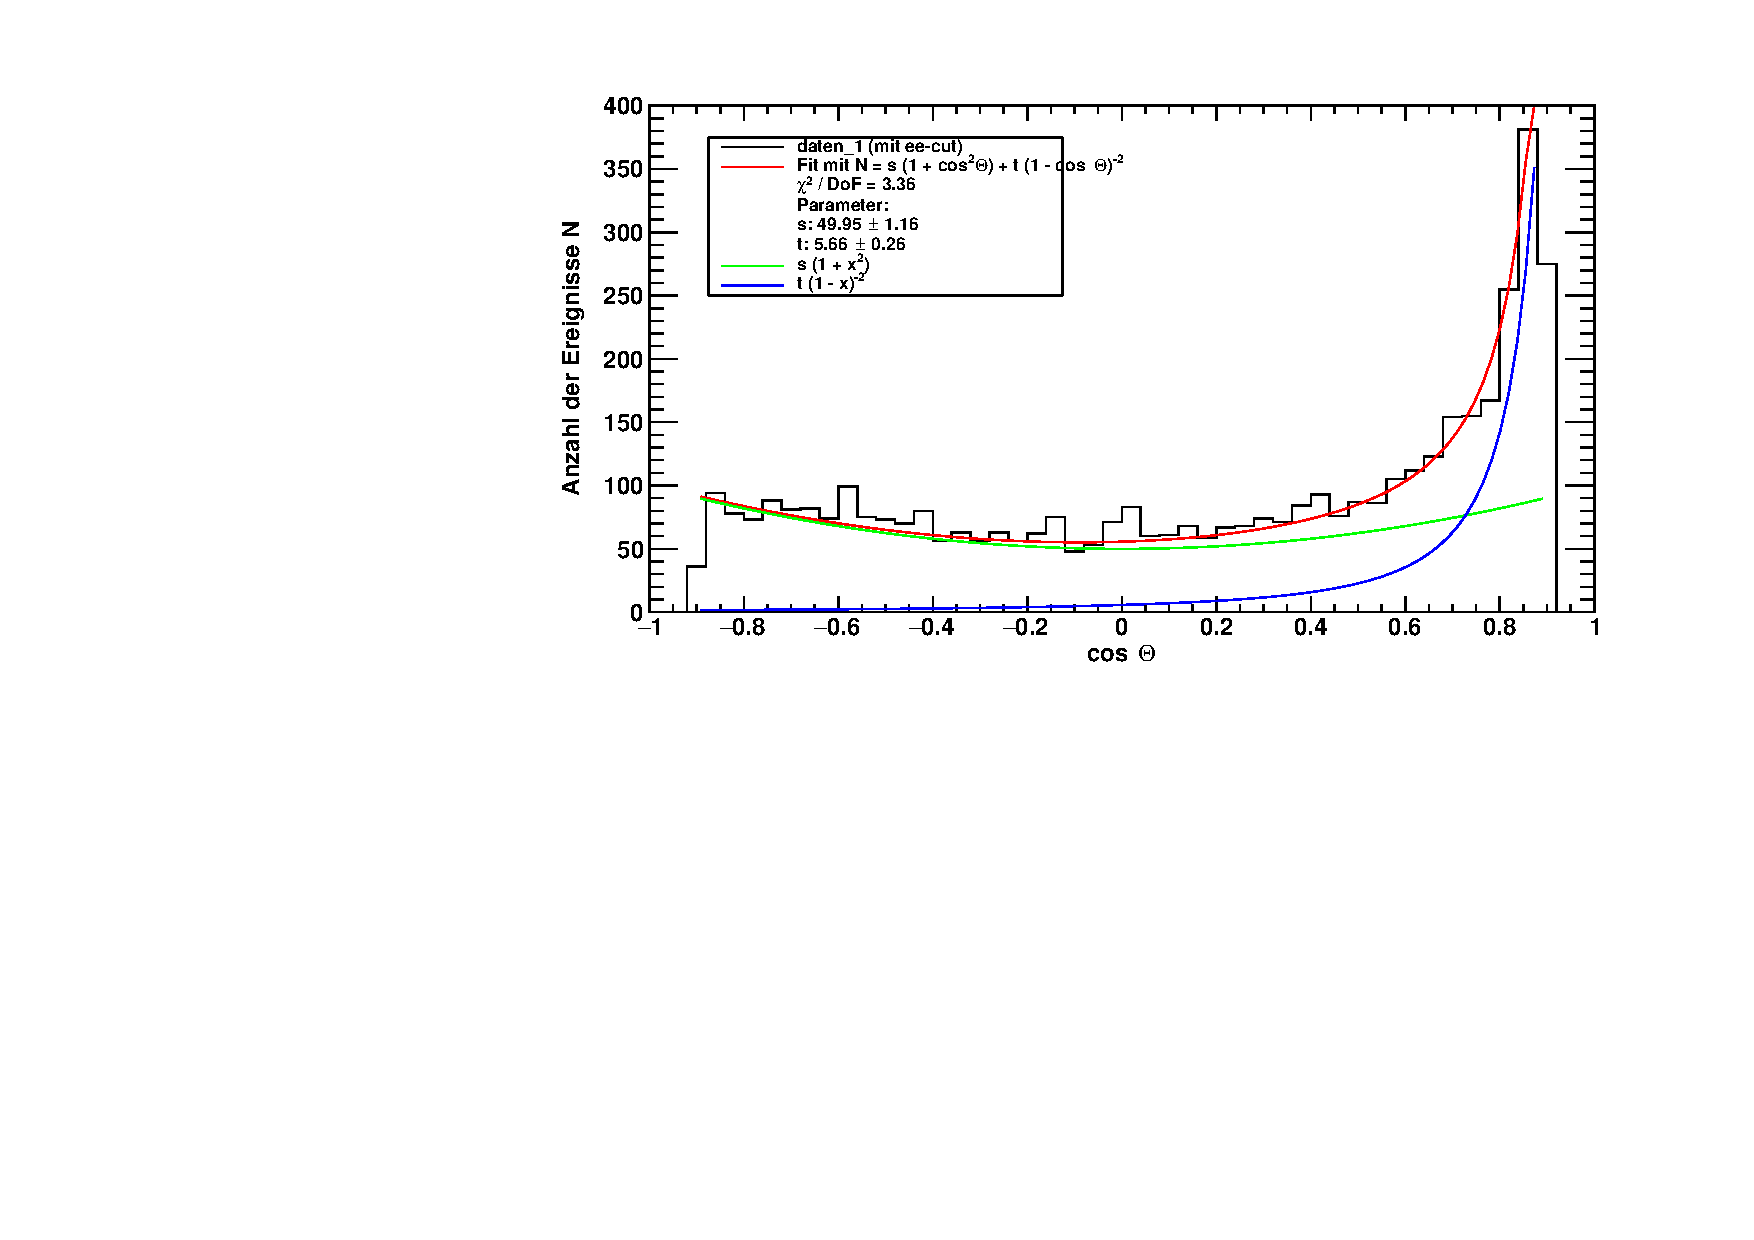
\includegraphics[width=\textwidth]{../img/s_t_fit_91-23.pdf}
  \caption{s-t-fit bei \sE{91.23}.}
  \label{img:label}
\end{center}
\end{figure}

\subsection{Auswertung der Wirkungsquerschnitte}
\begin{figure}[H]
\begin{center}
  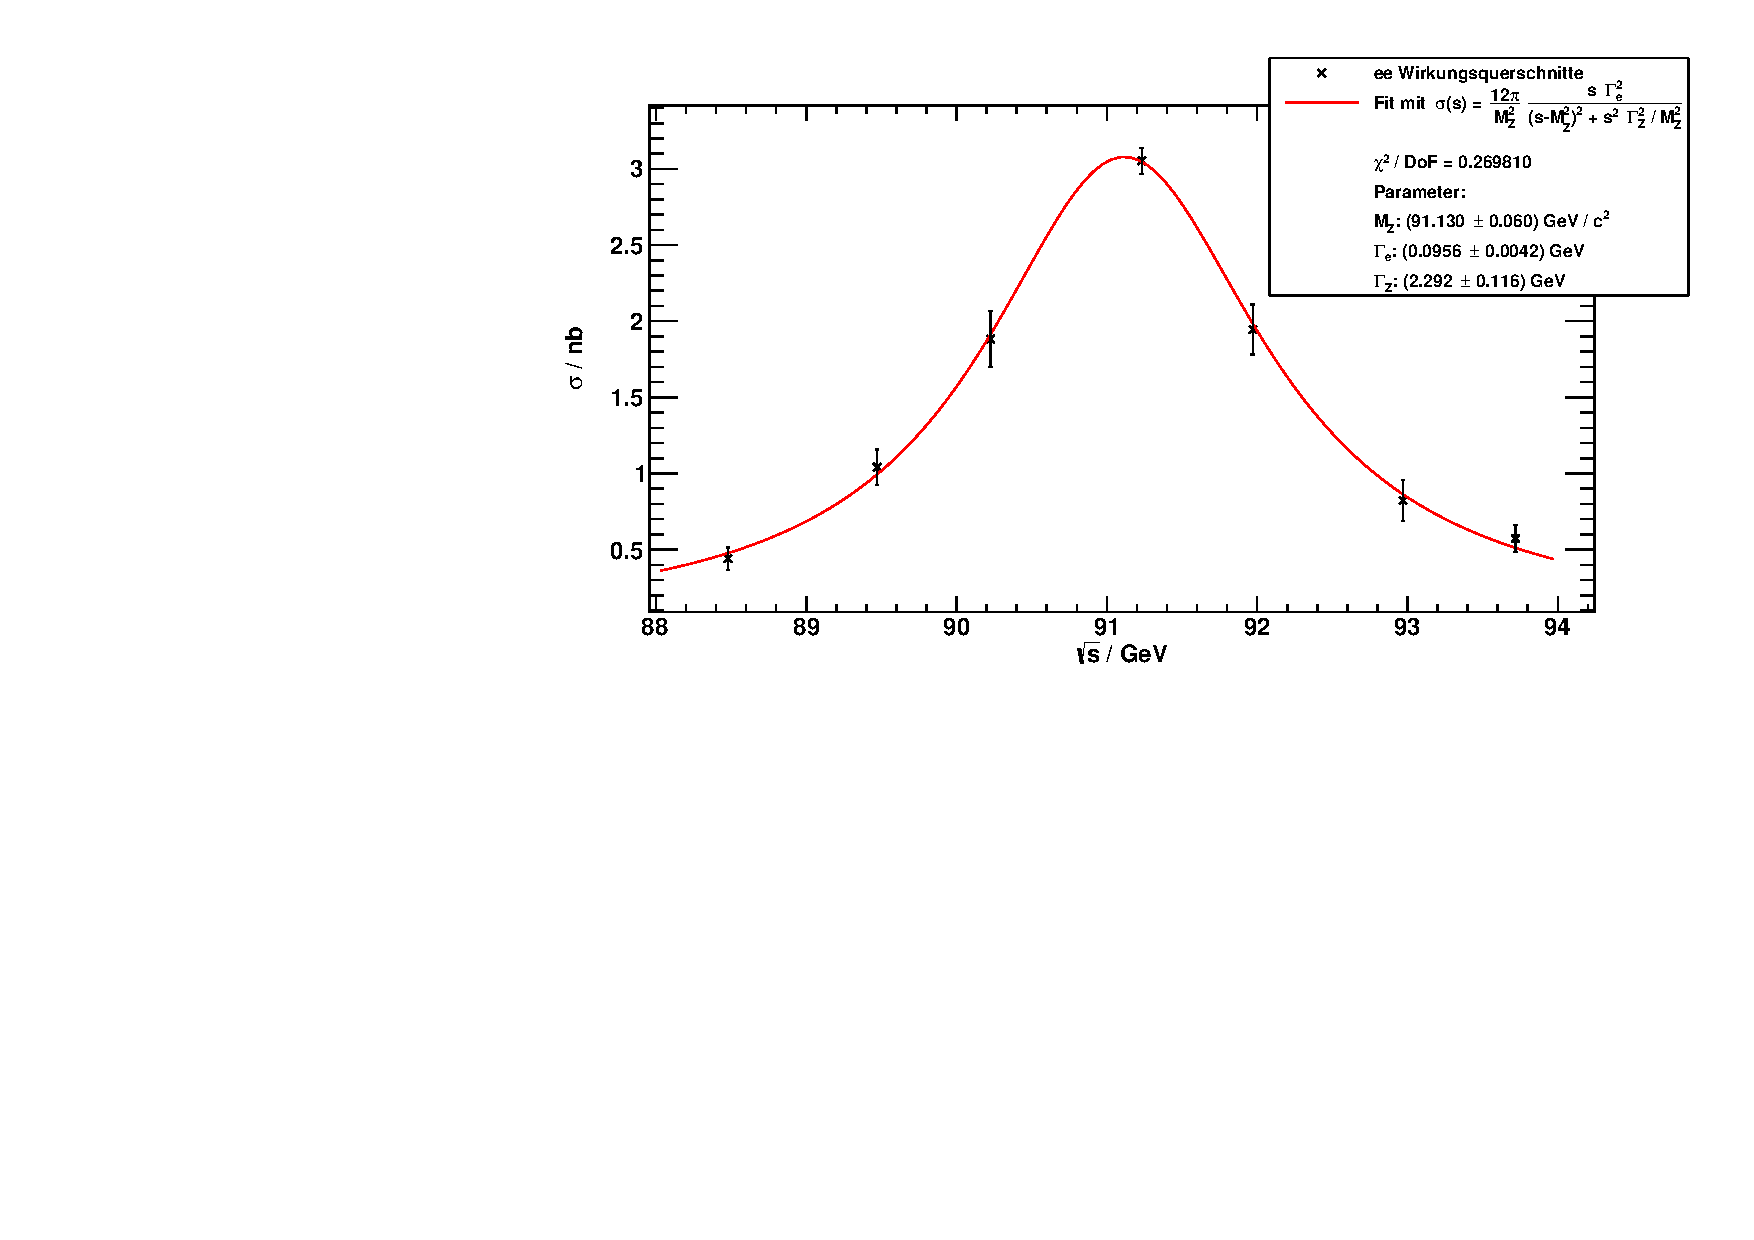
\includegraphics[width=\textwidth]{../img/crosssections_ee.pdf}
  \caption{Wirkungsquerschnitt für \ee $\to$ \ee.}
  \label{img:crosssection:ee}
\end{center}
\end{figure}

\begin{figure}[H]
\begin{center}
  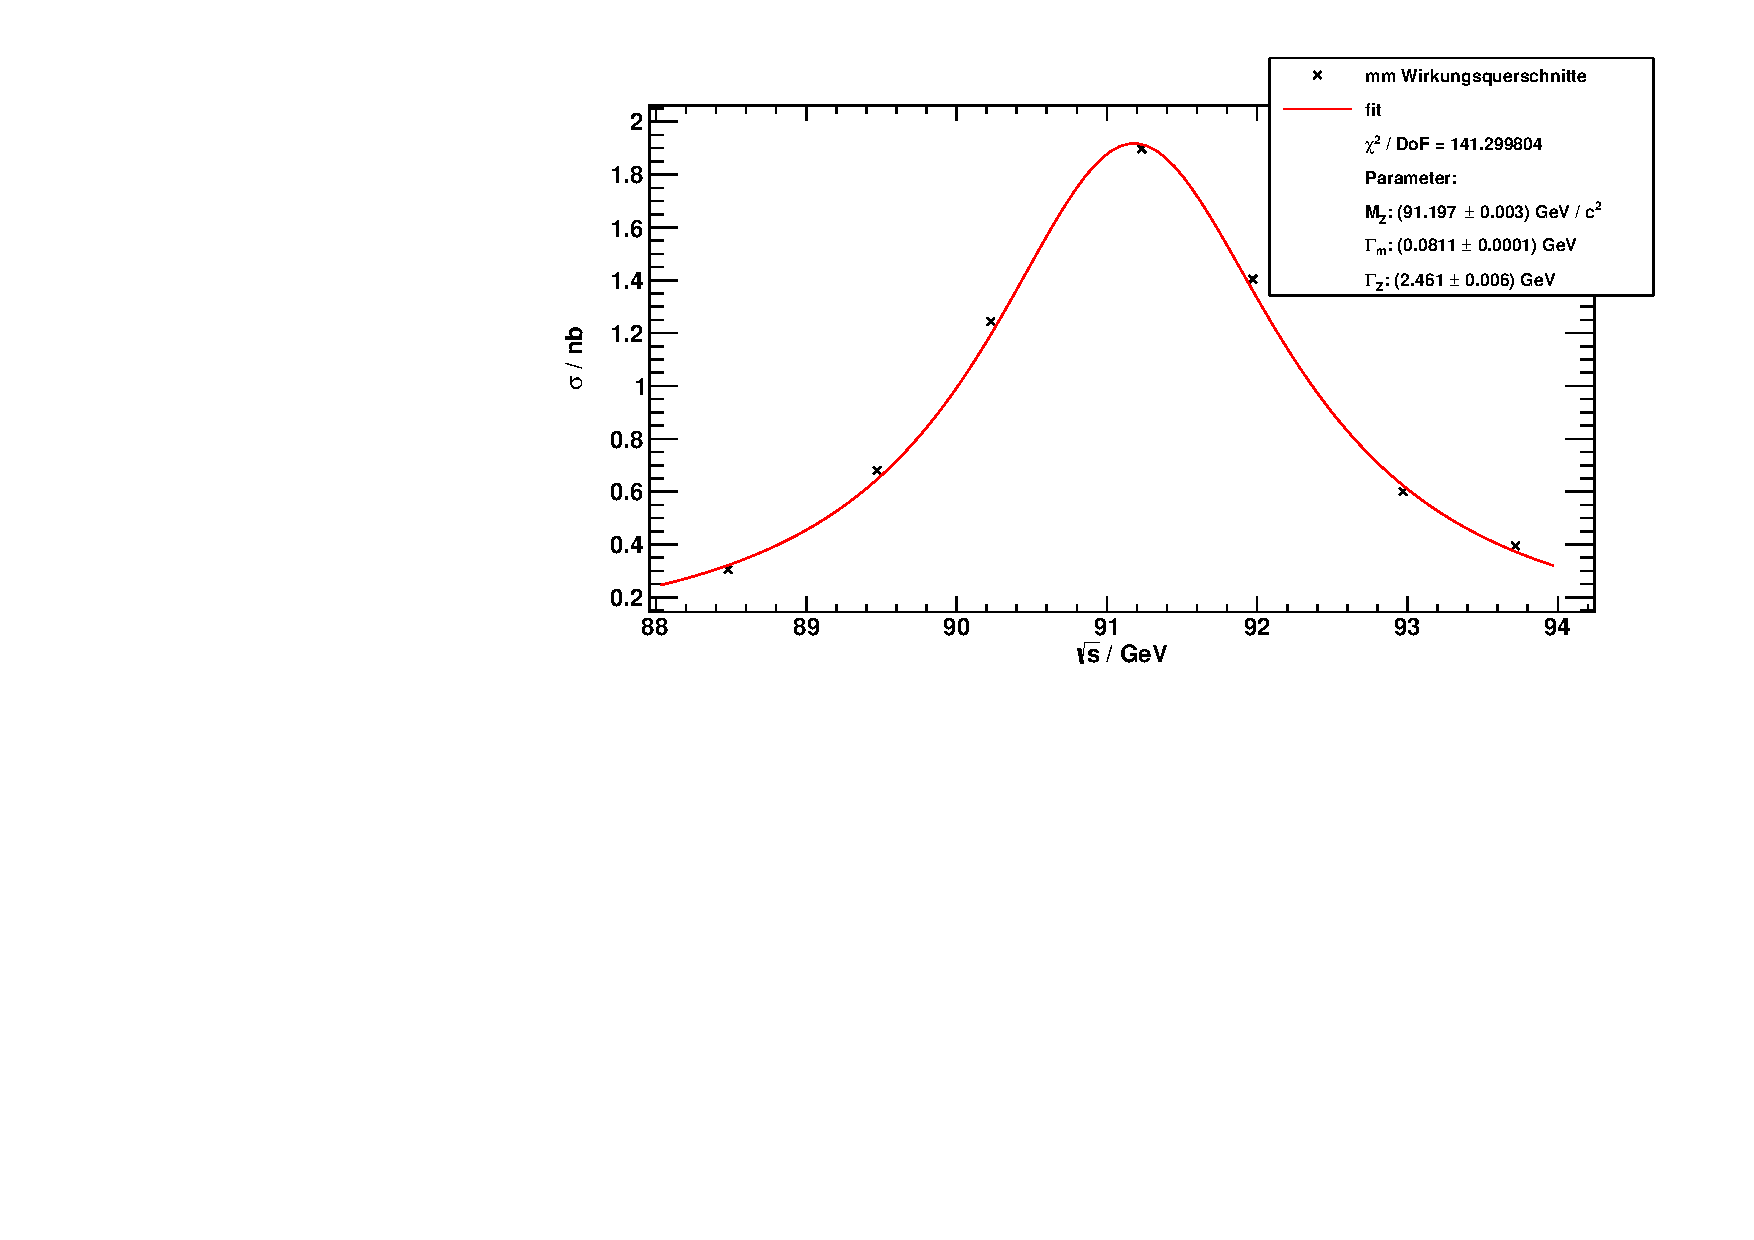
\includegraphics[width=\textwidth]{../img/crosssections_mm.pdf}
  \caption{Wirkungsquerschnitt für \ee $\to$ \mm.}
  \label{img:crosssection:mm}
\end{center}
\end{figure}

\begin{figure}[H]
\begin{center}
  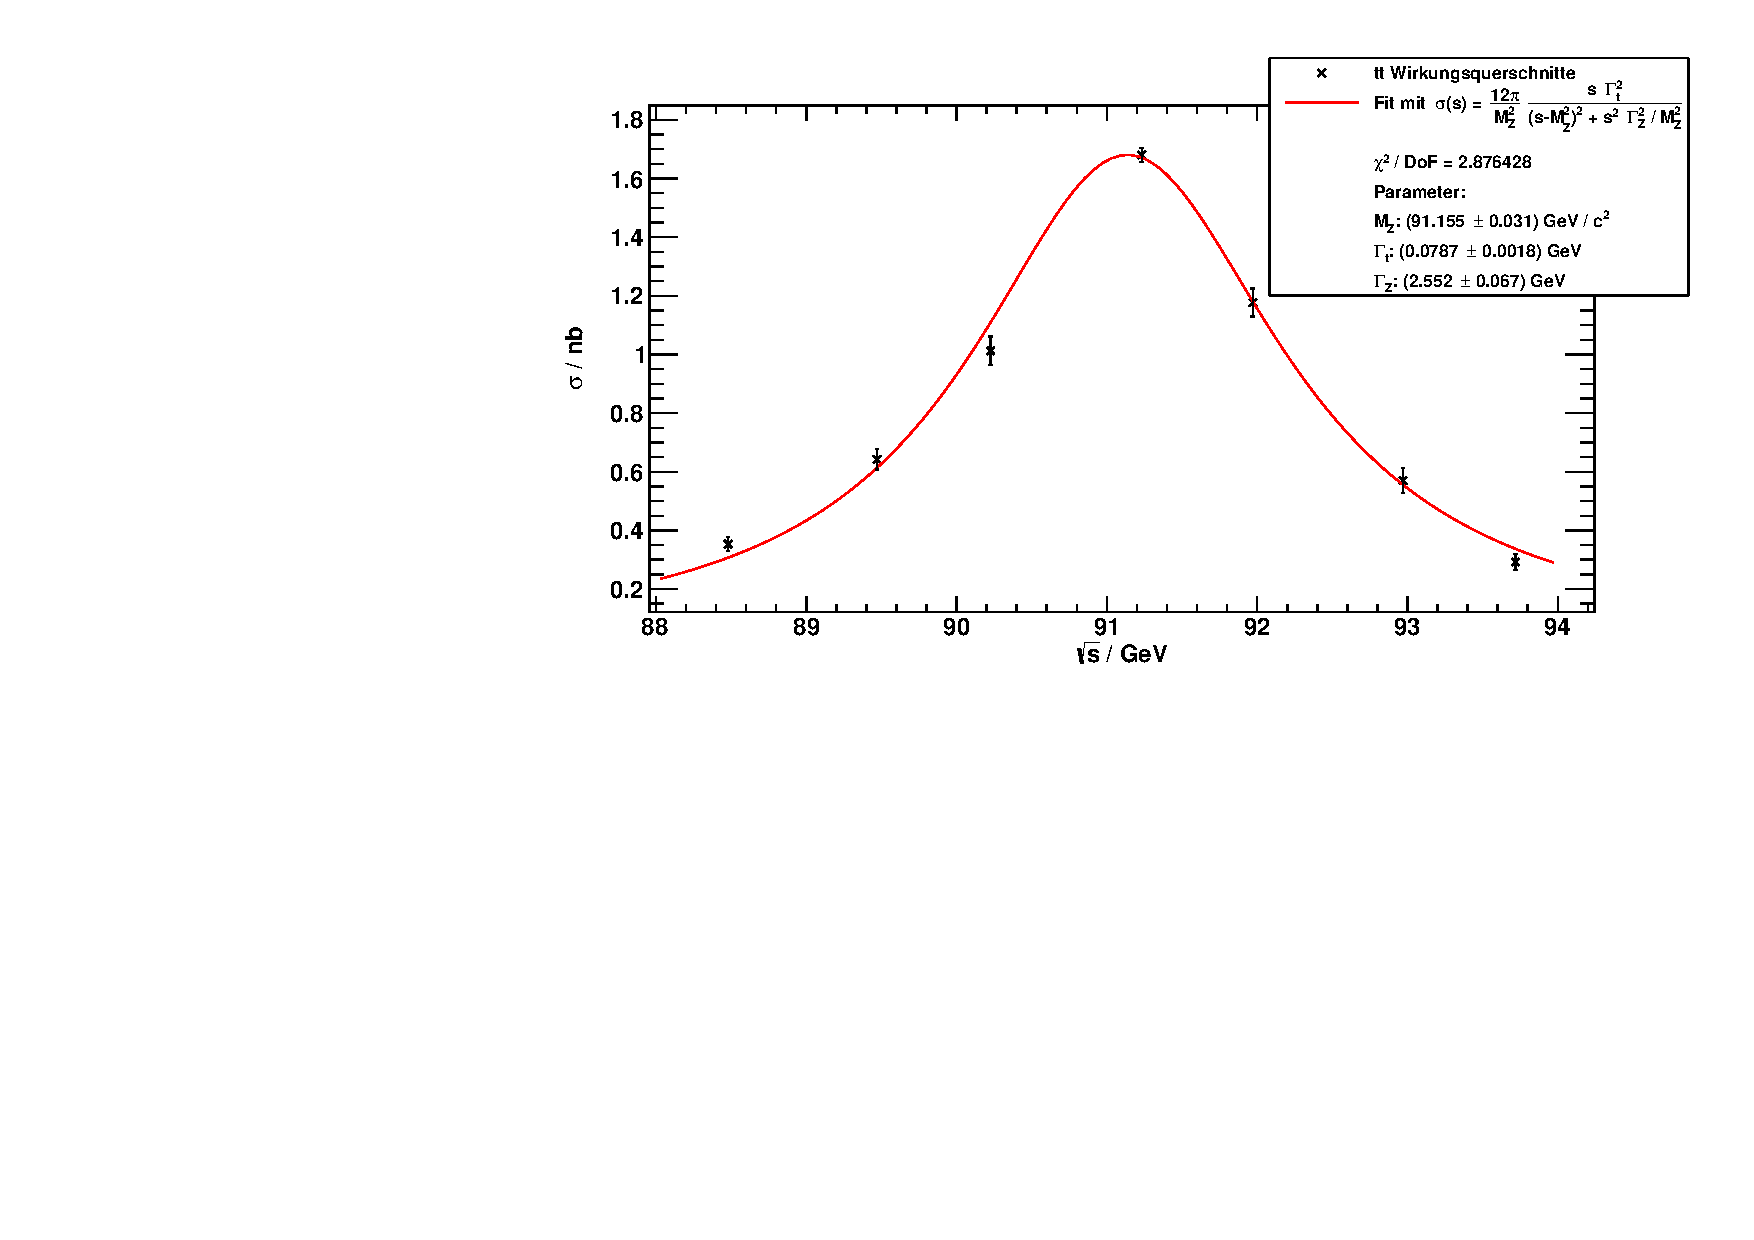
\includegraphics[width=\textwidth]{../img/crosssections_tt.pdf}
  \caption{Wirkungsquerschnitt für \ee $\to$ \tt.}
  \label{img:crosssection:tt}
\end{center}
\end{figure}

\begin{figure}[H]
\begin{center}
  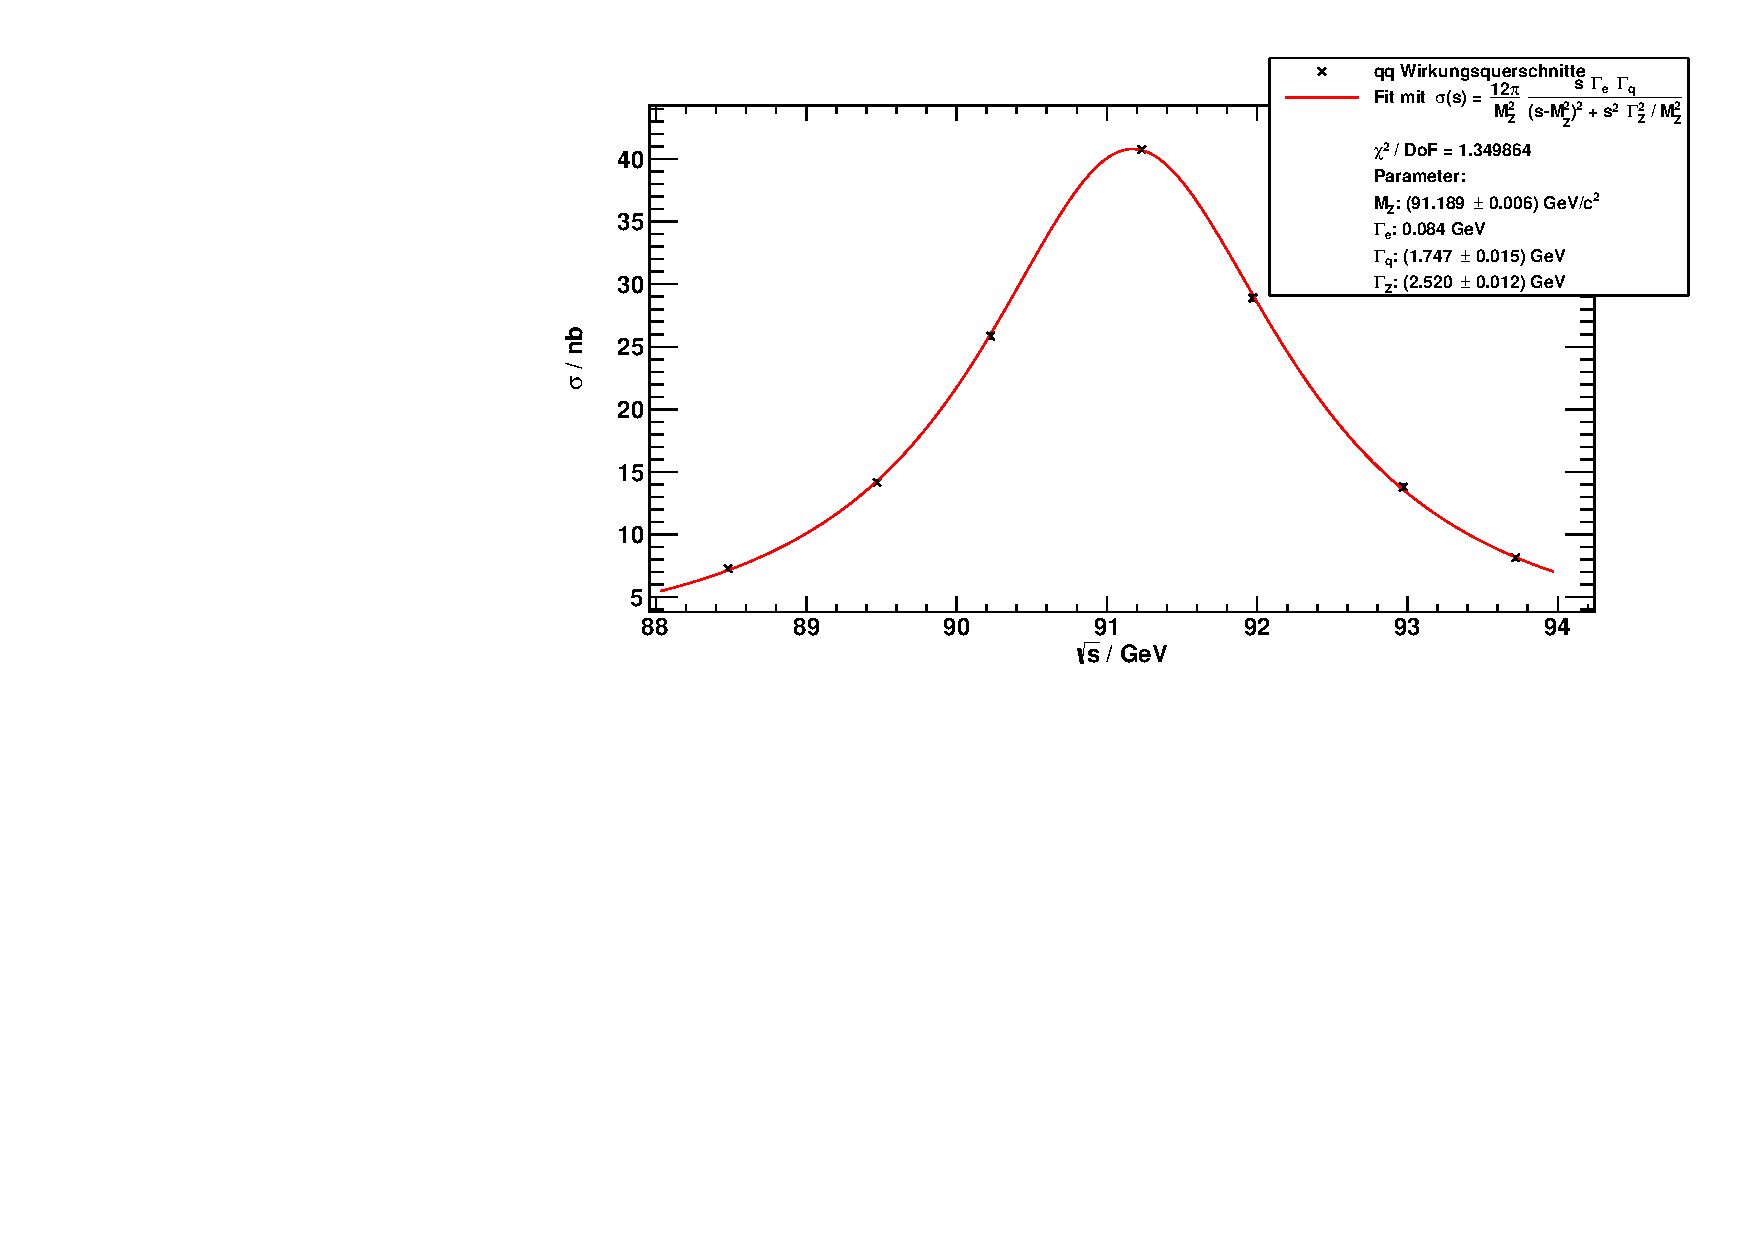
\includegraphics[width=\textwidth]{../img/crosssections_qq.pdf}
  \caption{Wirkungsquerschnitt für \ee $\to$ \qq.}
  \label{img:crosssection:qq}
\end{center}
\end{figure}

\subsubsection{Masse}
\subsubsection{Totale Zerfallsbreite}
\subsubsection{Partielle Zerfallsbreiten}
Leptonenuniversalität
\subsubsection{Anzahl leichter Neutrinogenerationen}
\subsection{Vorwärts-Rückwärts Asymmetrie}

Zitat BRs \cite{pdg}.